%\newpage
\section{Datamining} \label{sec:datamining}
The first step in the process of data mining is to decide on a fitting algorithmm. Because the best algorithm is not known in advance multiple are tested. For this project these were: KNNeighbors, Random Forest, Decision Tree, SVC, logistic regression, XGBoost, and four naïve bayes classifiers based on bernoulli, complement, gaussian  and multinomial.

These ten classification algorithms will be evaluated to determine which one yields the best results. The quality of an algorithm is determined by two properties. The first criterion is a high recall, in order to avoid possible Type 2 errors (a patient with a heart disease is diagnosed as negative) in the diagnosis. The second criterion is the number of examinations required. The reason for this is that we want our model to be universally used by doctors. We assume that this is especially the case when even simple examinations yield a good diagnosis. This criterion also corresponds to Occam’s Razor.

Besides the before mentioned use of scalers, imputers and samplers we additionally apply a variety of classifier specific hyperparameters. For the KNN we added the number of used neighbors from 2 to 97 moving in 5-unit steps as well as the distance metric L1 and L2 as hyperparameters. Random Forest was tested with 10 to 90 (10-unit steps) estimators and a maximum depth of None, 2, 6 and 10 and a minimum split of 2, 6, and 10. Decisions Trees were tested with both the gini index and entropy as impurity measures while the values for maximum tree depth and minimum split were the same as for Random Forest. In the case of logistic regression, we added the same distance options as for KNN. For SVC we tested C values ranging from 120 to 160 (20-unit steps), in combination with the gamma values 0.0001, 0.001, 0.01 and the kernel options linear, polynomial, sigmoidal and radial basis function. For the four naïve bayes estimators we applied alpha values from 0 to 19.5 (0.5-unit steps).

In order to find the best model a stratified nested cross validation was conducted using 10-folds each. To later decide which model was the best a classification report for every outer loop of the CV was saved. To run all CVs the work was split into several small parts where every unique combination of estimator, scaler and imputer represents its own part that was run on its own. This leads to 210 seperate cross validations. In the following evaluation only the best model according to the previously defined criterions (high recall and simplicity) for each estimator is reviewed in greater detail. For measuring the simplicity the minimum percentage to be dropped was used as a metric. If models performed equally we followed Occam's Razor and favoured models with a low number of columns and basic preprocessing. The results for every model can be seen in \cref{table:modelresults} in addition to some further prediction metrics without any ordering.


% INSERT TABLE

\begin{table}[]
	% \begin{adjustwidth}{-3cm}{}

	\begin{footnotesize}
		\begin{tabular}{|l|l|l|l|l|l|l|l|}
			\hline
			\textbf{Classifier} & \textbf{Scaler}  & \textbf{Sampler} & \textbf{Rec.} & \textbf{Rec. Std.} & \textbf{AUC.} & \textbf{F1} & \textbf{MPD} \\ \hline
			Baseline            & none             & none             & 1             & 0                  & 0.50         & 0.71        & 0            \\ \hline
			KNN                 & none             & none             & 0.85          & 0.04               & 0.76         & 0.80        & 0            \\ \hline
			XGB                 & Normalizer       & RUS              & 0.77          & 0.09               & 0.76         & 0.78        & 75           \\ \hline
			Random Forest       & StandardScaler   & none             & 0.84          & 0.09               & 0.78         & 0.81        & 100          \\ \hline
			Decision Tree       & none             & none             & 0.85          & 0.06               & 0.76         & 0.80        & 0            \\ \hline
			SVC                 & PowerTransformer & none             & 0.81          & 0.11               & 0.77         & 0.80        & 20           \\ \hline
			NB (bernoulli)      & StandardScaler   & none             & 0.79          & 0.08               & 0.76         & 0.79        & 8            \\ \hline
			NB (complement)     & MinMaxScaler     & none             & 0.84          & 0.03               & 0.77         & 0.81        & 100          \\ \hline
			NB (gaussian)       & Normalizer       & none             & 0.52          & 0.12               & 0.70         & 0.64        & 20           \\ \hline
			NB (multinomial)    & MinMaxScaler     & none             & 0.79          & 0.06               & 0.76         & 0.79        & 100          \\ \hline
			logistic regression & Normalizer       & none             & 0.84          & 0.07               & 0.76         & 0.80        & 0            \\ \hline
		\end{tabular}

		% \begin{adjustwidth}{+3cm}{}
		\begin{center}
			\centering
			RUS = random under sampler, MPD = minimum percentage to be dropped
		\end{center}
		% \end{adjustwidth}
	\end{footnotesize}
	\caption{Best models for every classification algorithm}
	\label{table:modelresults}

	% \end{adjustwidth}
\end{table}

The table includes all estimators as well as the baseline (majority vote). 

As the majority vote predicts a disease in all cases there are no false negatives and therefore the recall of our baseline is always 1. However, the model would not be usable in the real world because the doctors would not benefit from the prediction as the model would predict the same for every patient . This is why the table also includes AUC and F1 as comparison, where the trained models outperform the baseline. This makes all models better to use than the baseline, as they can provide real added value. 

In order to find the best model first the recall is analysed. Here larger differences can be observed. But the best performing models all have a recall of 0.84 to 0.85 (KNN, Random Forest, Descision Tree, NB (complete), logistic regression).  To further narrow down the selection, the simplicity of the models is considered on the basis of the MPD. Here the Random Forest and the NB model are excluded as they use all columns compared to the other models which only use completely filled columns. Since the remaining models do not differ significantly, a LeaveOneGroupOut cross validation is performed. Here, three data sets are used as the basis for training in order to classify the content of the fourth. The results for this procedure are also all within 0.01 for recall (0.78), precision (0.72), f1 (0.76), and accuracy (0.72). So they are assumed to be equal and Occam's Razor is conducted once more. KNN and the Decision Tree are simpler in preprocessing compared to the Logistic regression as they both do not use a scaler. If KNN and the Decision Tree are compared in their simplicity the Decision Tree outperforms the KNN because medical staff can just follow the decision tree where as a KNN computation can not be done easily. 

So we argue that the best model for classifying whether somebody has a heart disease or not is the model which uses the decision tree, followed closely by the before discussed KNN and logistic regression models.


The decision tree uses no scaler nor sampler. Also, no imputer was used because MPD is 0 and therefore no features with missing values remain. The best configuration was gini index as purity measure, a maximum tree depth of \texttt{None} and a minimum split of 2. This is identical to the defaults set by sklearn. 
In order to view what our best model assumes to be important indicators we have visualised the best decision tree model in \cref{fig:DecisionTree}. We only display the tree with depth 3 (total depth 5) since we aim at focusing on the main attributes. 
\begin{figure}[h]
	\centering
	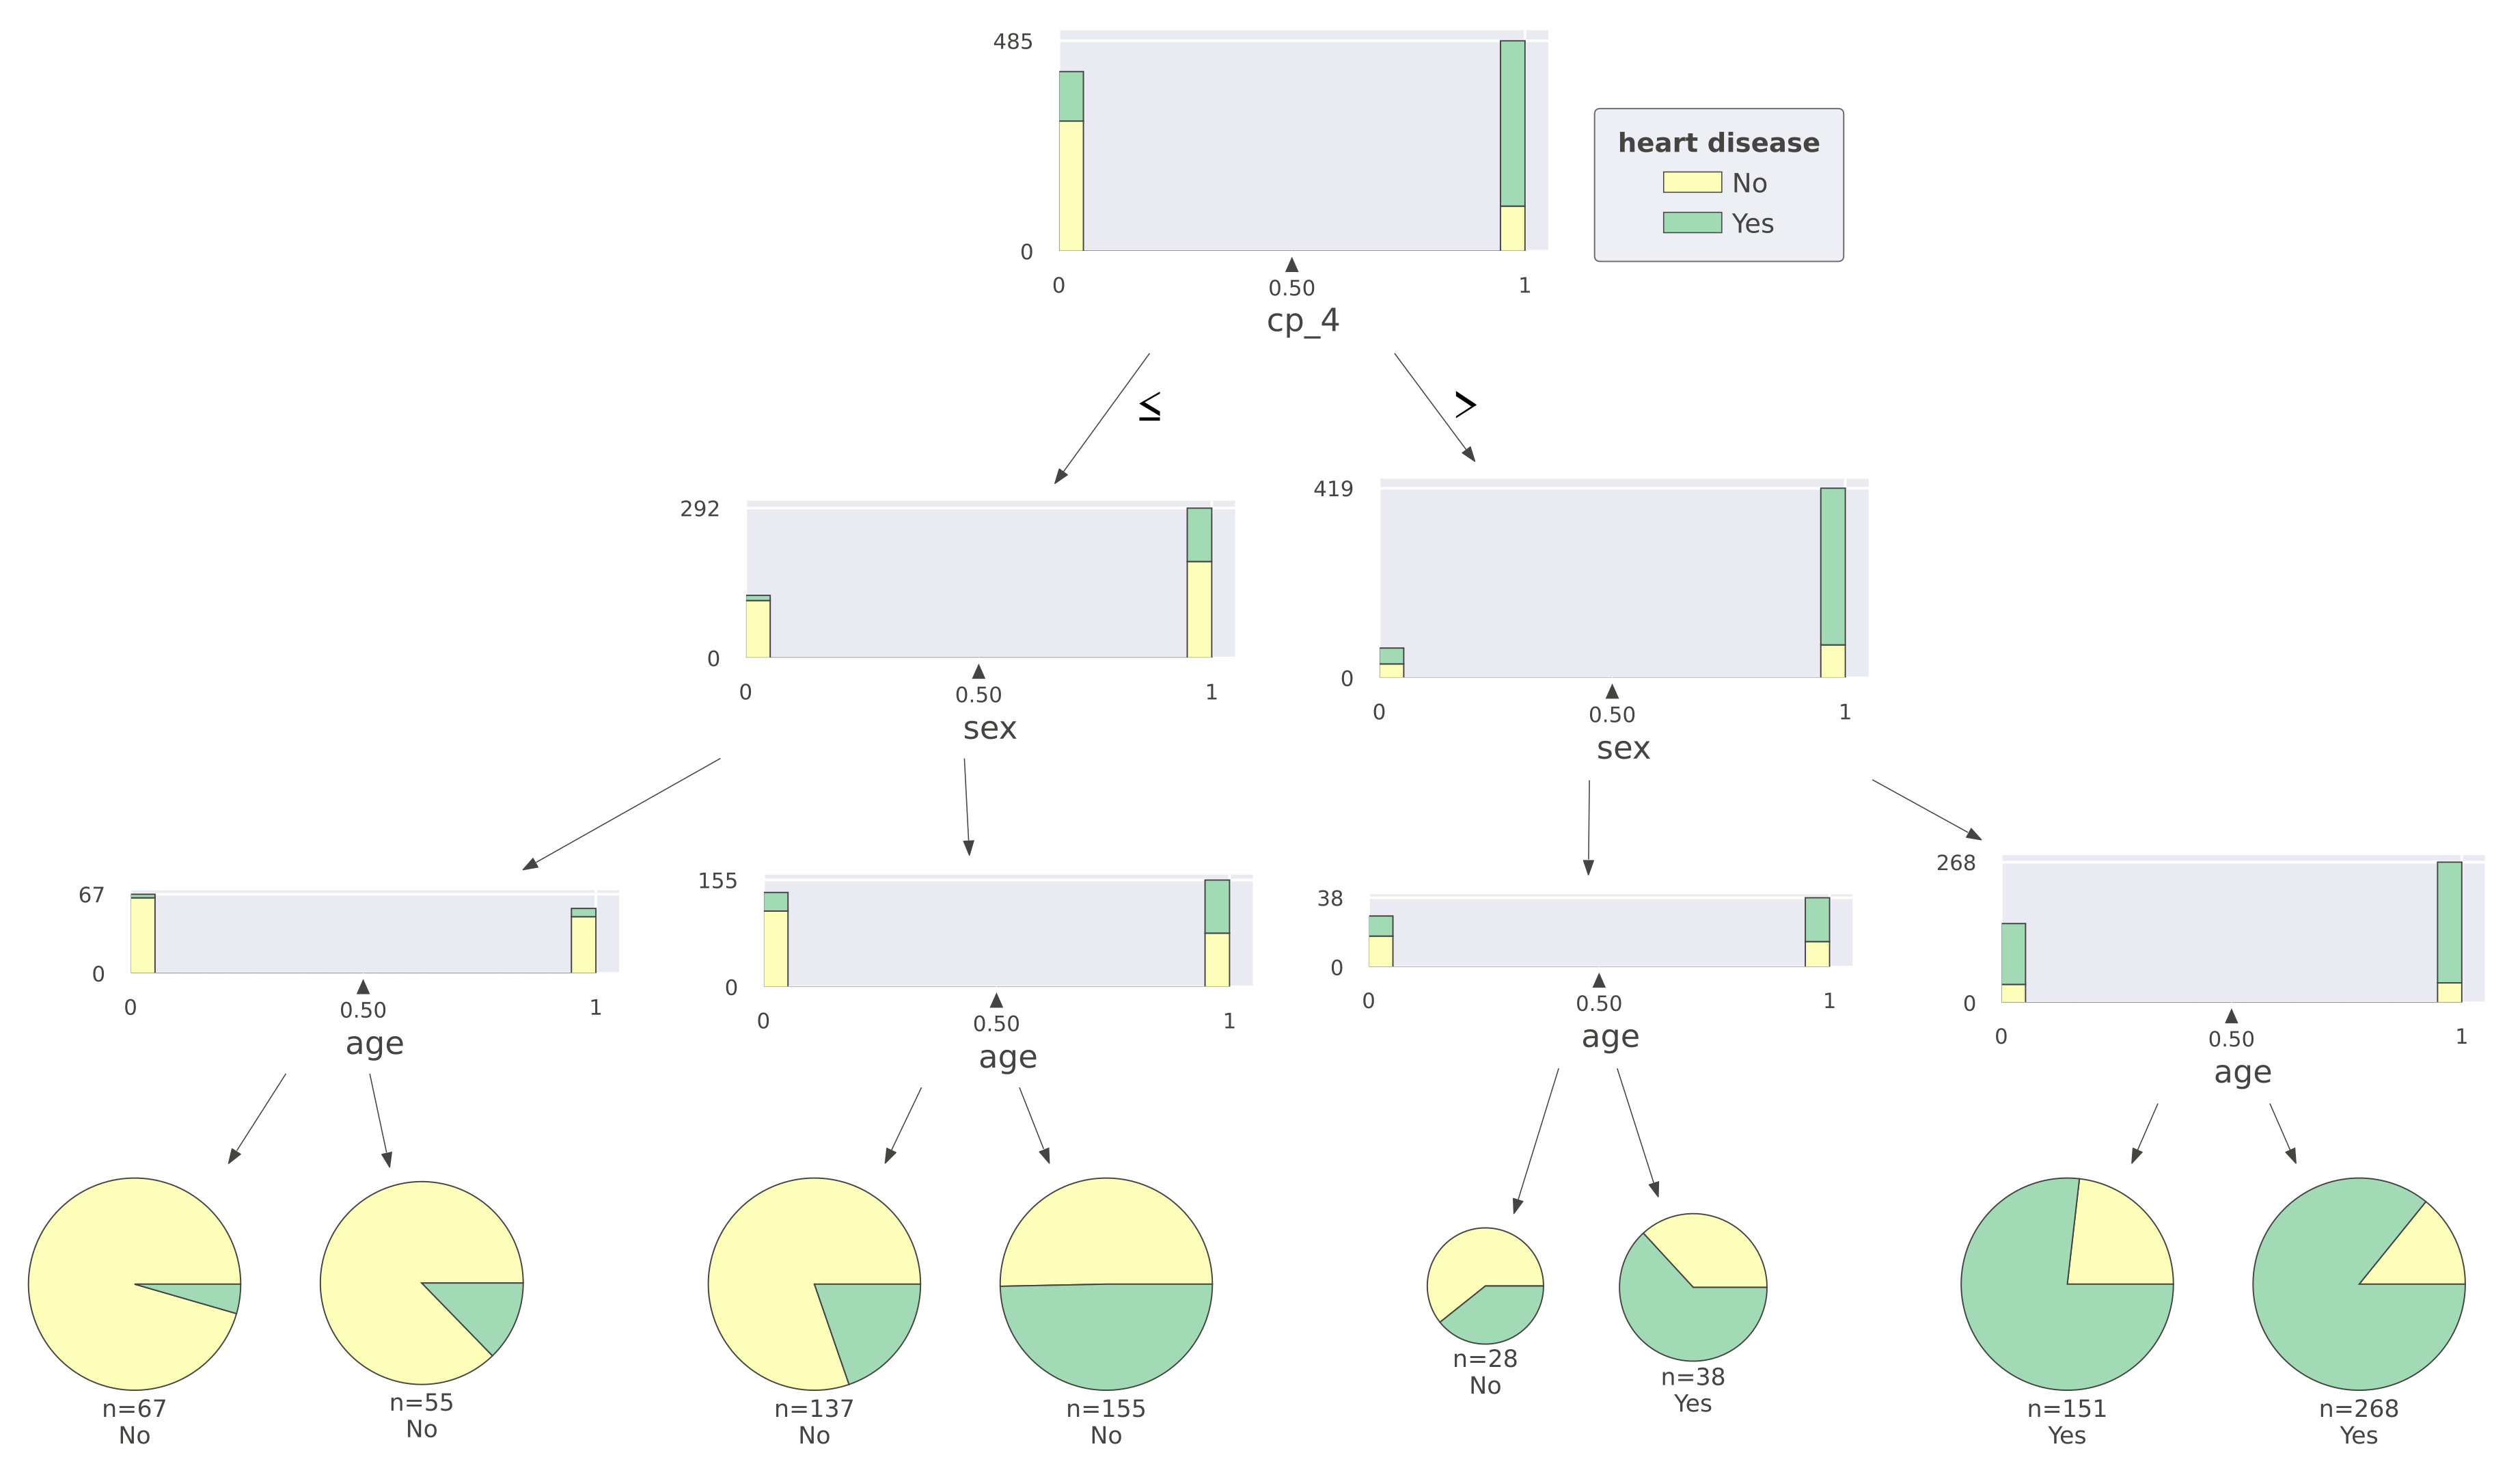
\includegraphics[width=0.7\textwidth]{images/DecisionTree.png}
	\caption{Decision tree visualized}
	\label{fig:DecisionTree}
\end{figure}

The root node of the tree decides whether a participant had asymptomatic chest pain or not. The resulting follow up nodes both use gender as the next split criterion. After that the tree splits according to age. The visualisation shows that older men with asymptomatic chest pain have the highest change to be predicted to have a heart disease. Overall, the model predicts men of all ages and with or without asymptomatic chest pain to have a higher probability of having a heart disease compared to women. The group with the lowest chance of having a heart disease are young women with no asymptomatic chest pain. The left side of the cp split conducts two more splits based on cp that are not displayed here. 